\documentclass[12pt]{article}


\usepackage{amssymb}
\usepackage{amsmath}
\usepackage{fullpage}
\usepackage{epsfig}
\usepackage{epstopdf}
\everymath{\displaystyle}
\usepackage{enumerate}



\begin{document}

\begin{center}
\underline{\LARGE{Chapter 3.3: Right Triangle Trigonometry}}
\end{center}

\subsection*{Expected Skills:}

\begin{itemize}

\item Be able to define evaluate $\sin{\theta}$, $\cos{\theta}$, $\tan{\theta}$, $\sec{\theta}$, $\csc{\theta}$, and $\cot{\theta}$ from a right triangle.

\end{itemize}

\subsection*{Practice Problems: }

\begin{enumerate}

\item Solve the following problems by drawing a triangle.

\begin{enumerate}

\item Find all possible values of $\sin{\theta}$ and $\cos{\theta}$ given that $\tan{\theta}=3$

\includegraphics[scale=0.5]{start.pdf}
{\begin{tabular}{l}
Since $\tan{\theta}>0$, the terminal side of $\theta$ is in either quadrant I or III.\\
If $\theta$ is in quadrant I: $\displaystyle \sin{\theta}=\frac{3}{\sqrt{10}}$ and $\displaystyle \cos{\theta}=\frac{1}{\sqrt{10}}$\\
If $\theta$ is in quadrant III: $\displaystyle \sin{\theta}=-\frac{3}{\sqrt{10}}$ and $\displaystyle \cos{\theta}=-\frac{1}{\sqrt{10}}$
\end{tabular}
}
\includegraphics[scale=0.5]{end.pdf}


\item Find all possible values of $\sin{\theta}$ and $\tan{\theta}$ given that $\displaystyle \cos{\theta}=\frac{2}{3}$

\includegraphics[scale=0.5]{start.pdf}
{\begin{tabular}{l}
Since $\cos{\theta}>0$, the terminal side of $\theta$ is in either quadrant I or IV.\\
If $\theta$ is in quadrant I: $\displaystyle \sin{\theta}=\frac{\sqrt{5}}{3}$ and $\displaystyle \tan{\theta}=\frac{\sqrt{5}}{2}$\\
If $\theta$ is in quadrant IV: $\displaystyle \sin{\theta}=-\frac{\sqrt{5}}{3}$ and $\displaystyle \tan{\theta}=-\frac{\sqrt{5}}{2}$\\
\end{tabular}
}
\includegraphics[scale=0.5]{end.pdf}


\item Find all possible values of $\tan{\theta}$ and $\csc{\theta}$ given that $\displaystyle \sec{\theta}=\frac{5}{2}$

\includegraphics[scale=0.5]{start.pdf}
{\begin{tabular}{l}
Since $\sec{\theta}>0$, the terminal side of $\theta$ is in either quadrant I or IV.\\
If $\theta$ is in quadrant I: $\displaystyle \tan{\theta}=\frac{\sqrt{21}}{2}$ and $\displaystyle \csc{\theta}=\frac{5}{\sqrt{21}}$\\
If $\theta$ is in quadrant IV: $\displaystyle \tan{\theta}=-\frac{\sqrt{21}}{2}$ and $\displaystyle \csc{\theta}=-\frac{5}{\sqrt{21}}$\\
\end{tabular}
}
\includegraphics[scale=0.5]{end.pdf}


\end{enumerate}

\item Compute the following:

\begin{enumerate}

\item $\displaystyle \cos{\theta}$ if $\displaystyle \sin{\theta}=-\frac{3}{5}$ and $\theta$ is in Quadrant IV.

\includegraphics[scale=0.5]{start.pdf}
{$\displaystyle \cos{\theta}=\frac{4}{5}$}
\includegraphics[scale=0.5]{end.pdf}


\item $\displaystyle \tan{\theta}$ if $\displaystyle \sec{\theta}=-\frac{9}{4}$ and $\theta$ is in Quadrant III.

\includegraphics[scale=0.5]{start.pdf}
{$\displaystyle \tan{\theta}=\frac{\sqrt{65}}{4}$}
\includegraphics[scale=0.5]{end.pdf}


\end{enumerate}

\item Use the given information to find the exact values of the remaining five trigonometric functions of $\theta$.

\begin{enumerate}

\item $\displaystyle \cos{\theta}=\frac{3}{5}$ and $\displaystyle 0 < \theta < \frac{\pi}{2}$

\includegraphics[scale=0.5]{start.pdf}
{$\displaystyle \sin{\theta}=\frac{4}{5}$, $\displaystyle \tan{\theta}=\frac{4}{3}$, $\displaystyle \sec{\theta}=\frac{5}{3}$, $\displaystyle \csc{\theta}=\frac{5}{4}$, and $\displaystyle \cot{\theta}=\frac{3}{4}$}
\includegraphics[scale=0.5]{end.pdf}


\item $\displaystyle \cos{\theta}=\frac{3}{5}$ and $\displaystyle -\frac{\pi}{2} < \theta < 0$

\includegraphics[scale=0.5]{start.pdf}
{$\displaystyle \sin{\theta}=-\frac{4}{5}$, $\displaystyle \tan{\theta}=-\frac{4}{3}$, $\displaystyle \sec{\theta}=\frac{5}{3}$, $\displaystyle \csc{\theta}=-\frac{5}{4}$, and $\displaystyle \cot{\theta}=-\frac{3}{4}$}
\includegraphics[scale=0.5]{end.pdf}


\item $\displaystyle \tan{\theta}=-\frac{1}{3}$ and $\displaystyle \frac{\pi}{2} < \theta < \pi$

\includegraphics[scale=0.5]{start.pdf}
{$\displaystyle \sin{\theta}=\frac{1}{\sqrt{10}}$, $\displaystyle \cos{\theta}=-\frac{3}{\sqrt{10}}$, $\displaystyle \sec{\theta}=-\frac{\sqrt{10}}{3}$, $\displaystyle \csc{\theta}=\sqrt{10}$, and $\displaystyle \cot{\theta}=-3$}
\includegraphics[scale=0.5]{end.pdf}


\item $\displaystyle \tan{\theta}=-\frac{1}{3}$ and $\displaystyle -\frac{\pi}{2} < \theta < 0$

\includegraphics[scale=0.5]{start.pdf}
{$\displaystyle \sin{\theta}=-\frac{1}{\sqrt{10}}$, $\displaystyle \cos{\theta}=\frac{3}{\sqrt{10}}$, $\displaystyle \sec{\theta}=\frac{\sqrt{10}}{3}$, $\displaystyle \csc{\theta}=-\sqrt{10}$, and $\displaystyle \cot{\theta}=-3$}
\includegraphics[scale=0.5]{end.pdf}


\item $\displaystyle \csc{\theta}=\sqrt{2}$ and $\displaystyle 0 < \theta < \frac{\pi}{2}$

\includegraphics[scale=0.5]{start.pdf}
{$\displaystyle \sin{\theta}=\frac{\sqrt{2}}{2}$, $\displaystyle \cos{\theta}=\frac{\sqrt{2}}{2}$, $\displaystyle \tan{\theta}=1$, $\displaystyle \sec{\theta}=\sqrt{2}$, and $\displaystyle \cot{\theta}=1$}
\includegraphics[scale=0.5]{end.pdf}


\item $\displaystyle \csc{\theta}=\sqrt{2}$ and $\displaystyle \frac{\pi}{2} < \theta < \pi$

\includegraphics[scale=0.5]{start.pdf}
{$\displaystyle \sin{\theta}=\frac{\sqrt{2}}{2}$, $\displaystyle \cos{\theta}=-\frac{\sqrt{2}}{2}$, $\displaystyle \tan{\theta}=-1$, $\displaystyle \sec{\theta}=-\sqrt{2}$, and $\displaystyle \cot{\theta}=-1$}
\includegraphics[scale=0.5]{end.pdf}


\end{enumerate}

\item A person is sitting in a Philadelphia movie theater waiting to watch the newest Star Wars movie.  He is sitting $d$ feet away from the screen.  The angle of elevation between his eyes and the bottom of the screen in $\alpha$ and the angle of elevation between his eyes and the top of the screen in is $\beta$, as in the diagram below.
\begin{center}
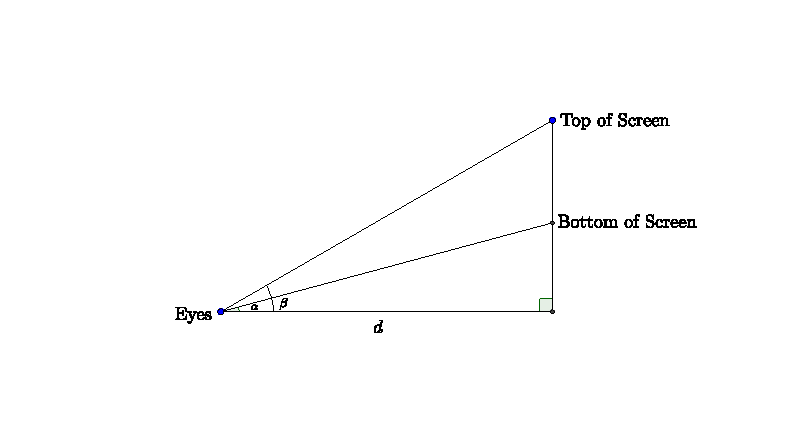
\includegraphics[scale=0.63]{screen.pdf}
\end{center}
Express the height of the screen in terms of $d$, $\alpha$, and $\beta$.

\includegraphics[scale=0.5]{start.pdf}
{$h=d\tan\beta-d\tan\alpha$ feet}
\includegraphics[scale=0.5]{end.pdf}


\newpage

\item Suppose $\theta$ is measured in radians and consider the following diagram:
\begin{center}
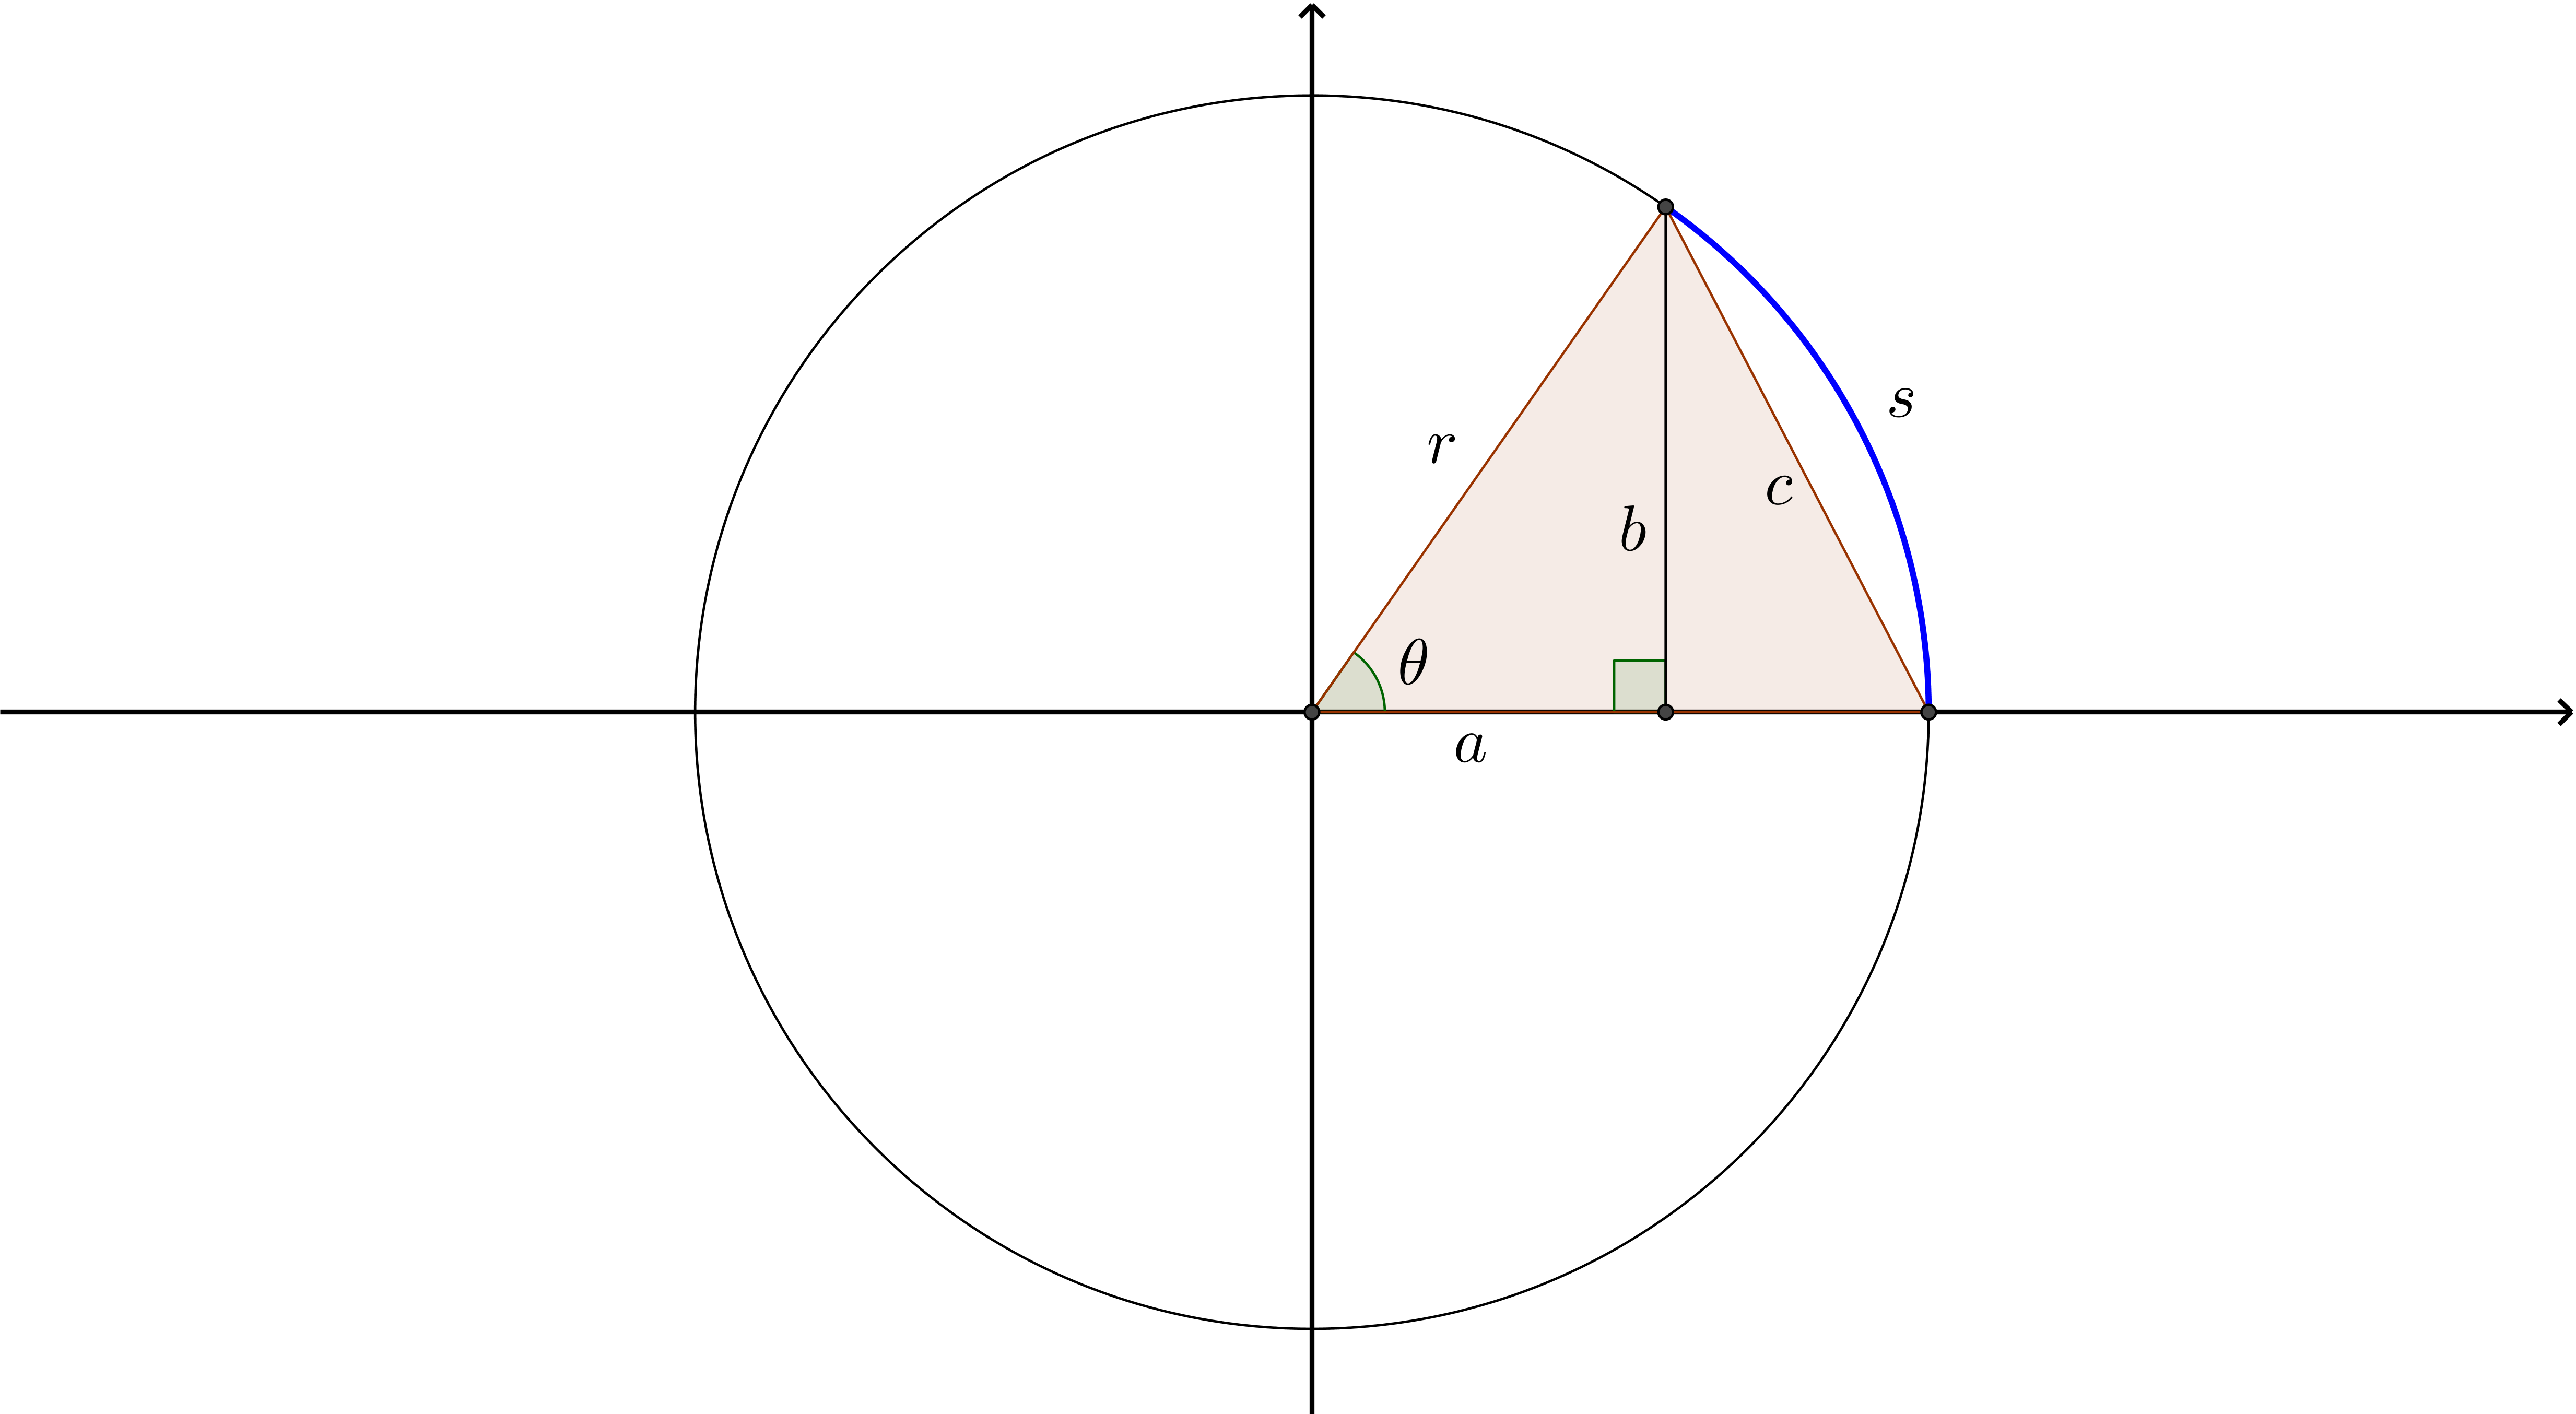
\includegraphics[scale=0.3]{circle.png}
\end{center}
Express $a$, $b$, and $c$ in terms of $r$ and $s$ only. (Your answers may involve trigonometric functions.)

\includegraphics[scale=0.5]{start.pdf}
{{{1\linewidth}{
Notice that $\theta = \frac{s}{r}$.  Then, $a=r\cos\left(\frac{s}{r}\right)$ and $b=r\sin\left(\frac{s}{r}\right)$.  Finally, with $a$ and $b$ as described, one can calculate $c=\sqrt{b^2+(r-a)^2}$.
}}}
\includegraphics[scale=0.5]{end.pdf}


\end{enumerate}

\end{document}